\documentclass[a4paper]{article}

\def\npart {IB}
\def\nterm {Lent}
\def\nyear {2016}
\def\nlecturer {R. E. Hunt}
\def\ncourse {Complex Methods}
\def\nlectures {MWF.9}
\def\nnotready {}

% Imports
\ifx \nextra \undefined
  \usepackage[pdftex,
    hidelinks,
    pdfauthor={Dexter Chua},
    pdfsubject={Cambridge Maths Notes: Part \npart\ - \ncourse},
    pdftitle={Part \npart\ - \ncourse},
  pdfkeywords={Cambridge Mathematics Maths Math \npart\ \nterm\ \nyear\ \ncourse}]{hyperref}
  \title{Part \npart\ - \ncourse}
\else
  \usepackage[pdftex,
    hidelinks,
    pdfauthor={Dexter Chua},
    pdfsubject={Cambridge Maths Notes: Part \npart\ - \ncourse\ (\nextra)},
    pdftitle={Part \npart\ - \ncourse\ (\nextra)},
  pdfkeywords={Cambridge Mathematics Maths Math \npart\ \nterm\ \nyear\ \ncourse\ \nextra}]{hyperref}

  \title{Part \npart\ - \ncourse \\ {\Large \nextra}}
\fi

\author{Lectured by \nlecturer \\\small Notes taken by Dexter Chua}
\date{\nterm\ \nyear}

\usepackage{alltt}
\usepackage{amsfonts}
\usepackage{amsmath}
\usepackage{amssymb}
\usepackage{amsthm}
\usepackage{booktabs}
\usepackage{caption}
\usepackage{enumitem}
\usepackage{fancyhdr}
\usepackage{graphicx}
\usepackage{mathtools}
\usepackage{microtype}
\usepackage{multirow}
\usepackage{pdflscape}
\usepackage{pgfplots}
\usepackage{siunitx}
\usepackage{tabularx}
\usepackage{tikz}
\usepackage{tkz-euclide}
\usepackage[normalem]{ulem}
\usepackage[all]{xy}

\pgfplotsset{compat=1.12}

\pagestyle{fancyplain}
\lhead{\emph{\nouppercase{\leftmark}}}
\ifx \nextra \undefined
  \rhead{
    \ifnum\thepage=1
    \else
      \npart\ \ncourse
    \fi}
\else
  \rhead{
    \ifnum\thepage=1
    \else
      \npart\ \ncourse\ (\nextra)
    \fi}
\fi
\usetikzlibrary{arrows}
\usetikzlibrary{decorations.markings}
\usetikzlibrary{decorations.pathmorphing}
\usetikzlibrary{positioning}
\usetikzlibrary{fadings}
\usetikzlibrary{intersections}
\usetikzlibrary{cd}

\newcommand*{\Cdot}{\raisebox{-0.25ex}{\scalebox{1.5}{$\cdot$}}}
\newcommand {\pd}[2][ ]{
  \ifx #1 { }
    \frac{\partial}{\partial #2}
  \else
    \frac{\partial^{#1}}{\partial #2^{#1}}
  \fi
}

% Theorems
\theoremstyle{definition}
\newtheorem*{aim}{Aim}
\newtheorem*{axiom}{Axiom}
\newtheorem*{claim}{Claim}
\newtheorem*{cor}{Corollary}
\newtheorem*{defi}{Definition}
\newtheorem*{eg}{Example}
\newtheorem*{fact}{Fact}
\newtheorem*{law}{Law}
\newtheorem*{lemma}{Lemma}
\newtheorem*{notation}{Notation}
\newtheorem*{prop}{Proposition}
\newtheorem*{thm}{Theorem}

\renewcommand{\labelitemi}{--}
\renewcommand{\labelitemii}{$\circ$}
\renewcommand{\labelenumi}{(\roman{*})}

\let\stdsection\section
\renewcommand\section{\newpage\stdsection}

% Strike through
\def\st{\bgroup \ULdepth=-.55ex \ULset}

% Maths symbols
\newcommand{\bra}{\langle}
\newcommand{\ket}{\rangle}

\newcommand{\N}{\mathbb{N}}
\newcommand{\Z}{\mathbb{Z}}
\newcommand{\Q}{\mathbb{Q}}
\renewcommand{\H}{\mathbb{H}}
\newcommand{\R}{\mathbb{R}}
\newcommand{\C}{\mathbb{C}}
\newcommand{\Prob}{\mathbb{P}}
\renewcommand{\P}{\mathbb{P}}
\newcommand{\E}{\mathbb{E}}
\newcommand{\F}{\mathbb{F}}
\newcommand{\cU}{\mathcal{U}}
\newcommand{\RP}{\mathbb{RP}}
\newcommand{\CP}{\mathbb{CP}}

\newcommand{\ph}{\,\cdot\,}

\DeclareMathOperator{\sech}{sech}
\DeclareMathOperator{\cosech}{cosech}
\DeclareMathOperator{\cosec}{cosec}

\DeclareMathOperator{\covol}{covol}
\DeclareMathOperator{\vol}{vol}

\let\Im\relax
\let\Re\relax
\DeclareMathOperator{\Im}{Im}
\DeclareMathOperator{\Re}{Re}
\DeclareMathOperator{\im}{im}
\DeclareMathOperator{\image}{image}
\DeclareMathOperator{\Ann}{Ann}

\DeclareMathOperator*{\res}{res}
\DeclareMathOperator{\Res}{Res}
\DeclareMathOperator{\Ind}{Ind}

\DeclareMathOperator{\tr}{tr}
\DeclareMathOperator{\diag}{diag}
\DeclareMathOperator{\rank}{rank}
\DeclareMathOperator{\card}{card}
\DeclareMathOperator{\spn}{span}
\DeclareMathOperator{\adj}{adj}

\DeclareMathOperator{\erf}{erf}
\DeclareMathOperator{\erfc}{erfc}

\DeclareMathOperator{\ord}{ord}
\DeclareMathOperator{\Sym}{Sym}

\DeclareMathOperator{\sgn}{sgn}
\DeclareMathOperator{\orb}{orb}
\DeclareMathOperator{\stab}{stab}
\DeclareMathOperator{\ccl}{ccl}

\DeclareMathOperator{\lcm}{lcm}
\DeclareMathOperator{\hcf}{hcf}

\DeclareMathOperator{\Int}{Int}
\DeclareMathOperator{\id}{id}

\DeclareMathOperator{\betaD}{beta}
\DeclareMathOperator{\gammaD}{gamma}
\DeclareMathOperator{\Poisson}{Poisson}
\DeclareMathOperator{\binomial}{binomial}
\DeclareMathOperator{\multinomial}{multinomial}
\DeclareMathOperator{\Bernoulli}{Bernoulli}
\DeclareMathOperator{\like}{like}

\DeclareMathOperator{\var}{var}
\DeclareMathOperator{\cov}{cov}
\DeclareMathOperator{\bias}{bias}
\DeclareMathOperator{\mse}{mse}
\DeclareMathOperator{\corr}{corr}

\DeclareMathOperator{\otp}{otp}
\DeclareMathOperator{\dom}{dom}

\DeclareMathOperator{\Root}{Root}
\DeclareMathOperator{\supp}{supp}
\DeclareMathOperator{\rel}{rel}
\DeclareMathOperator{\Hom}{Hom}
\DeclareMathOperator{\Aut}{Aut}
\DeclareMathOperator{\Gal}{Gal}
\DeclareMathOperator{\Mat}{Mat}
\DeclareMathOperator{\End}{End}
\DeclareMathOperator{\Char}{char}
\DeclareMathOperator{\ev}{ev}
\DeclareMathOperator{\St}{St}
\DeclareMathOperator{\Lk}{Lk}
\DeclareMathOperator{\disc}{disc}
\DeclareMathOperator{\Isom}{Isom}
\DeclareMathOperator{\length}{length}
\DeclareMathOperator{\energy}{energy}
\DeclareMathOperator{\area}{area}
\DeclareMathOperator{\Syl}{Syl}
\DeclareMathOperator{\cl}{cl}
\DeclareMathOperator{\fix}{fix}

\newcommand{\GL}{\mathrm{GL}}
\newcommand{\SL}{\mathrm{SL}}
\newcommand{\PGL}{\mathrm{PGL}}
\newcommand{\PSL}{\mathrm{PSL}}
\newcommand{\PSU}{\mathrm{PSU}}
\newcommand{\Or}{\mathrm{O}}
\newcommand{\SO}{\mathrm{SO}}
\newcommand{\U}{\mathrm{U}}
\newcommand{\SU}{\mathrm{SU}}

\renewcommand{\d}{\mathrm{d}}
\newcommand{\D}{\mathrm{D}}

\tikzset{->/.style = {decoration={markings,
                                  mark=at position 1 with {\arrow[scale=2]{latex'}}},
                      postaction={decorate}}}
\tikzset{<-/.style = {decoration={markings,
                                  mark=at position 0 with {\arrowreversed[scale=2]{latex'}}},
                      postaction={decorate}}}
\tikzset{<->/.style = {decoration={markings,
                                   mark=at position 0 with {\arrowreversed[scale=2]{latex'}},
                                   mark=at position 1 with {\arrow[scale=2]{latex'}}},
                       postaction={decorate}}}
\tikzset{->-/.style = {decoration={markings,
                                   mark=at position #1 with {\arrow[scale=2]{latex'}}},
                       postaction={decorate}}}
\tikzset{-<-/.style = {decoration={markings,
                                   mark=at position #1 with {\arrowreversed[scale=2]{latex'}}},
                       postaction={decorate}}}

\tikzset{circ/.style = {fill, circle, inner sep = 0, minimum size = 3}}
\tikzset{mstate/.style={circle, draw, blue, text=black, minimum width=0.7cm}}

\definecolor{mblue}{rgb}{0.2, 0.3, 0.8}
\definecolor{morange}{rgb}{1, 0.5, 0}
\definecolor{mgreen}{rgb}{0.1, 0.4, 0.2}
\definecolor{mred}{rgb}{0.5, 0, 0}

\def\drawcirculararc(#1,#2)(#3,#4)(#5,#6){%
    \pgfmathsetmacro\cA{(#1*#1+#2*#2-#3*#3-#4*#4)/2}%
    \pgfmathsetmacro\cB{(#1*#1+#2*#2-#5*#5-#6*#6)/2}%
    \pgfmathsetmacro\cy{(\cB*(#1-#3)-\cA*(#1-#5))/%
                        ((#2-#6)*(#1-#3)-(#2-#4)*(#1-#5))}%
    \pgfmathsetmacro\cx{(\cA-\cy*(#2-#4))/(#1-#3)}%
    \pgfmathsetmacro\cr{sqrt((#1-\cx)*(#1-\cx)+(#2-\cy)*(#2-\cy))}%
    \pgfmathsetmacro\cA{atan2(#2-\cy,#1-\cx)}%
    \pgfmathsetmacro\cB{atan2(#6-\cy,#5-\cx)}%
    \pgfmathparse{\cB<\cA}%
    \ifnum\pgfmathresult=1
        \pgfmathsetmacro\cB{\cB+360}%
    \fi
    \draw (#1,#2) arc (\cA:\cB:\cr);%
}
\newcommand\getCoord[3]{\newdimen{#1}\newdimen{#2}\pgfextractx{#1}{\pgfpointanchor{#3}{center}}\pgfextracty{#2}{\pgfpointanchor{#3}{center}}}

\def\Xint#1{\mathchoice
   {\XXint\displaystyle\textstyle{#1}}%
   {\XXint\textstyle\scriptstyle{#1}}%
   {\XXint\scriptstyle\scriptscriptstyle{#1}}%
   {\XXint\scriptscriptstyle\scriptscriptstyle{#1}}%
   \!\int}
\def\XXint#1#2#3{{\setbox0=\hbox{$#1{#2#3}{\int}$}
     \vcenter{\hbox{$#2#3$}}\kern-.5\wd0}}
\def\ddashint{\Xint=}
\def\dashint{\Xint-}


\begin{document}
\maketitle
{\small
\noindent\textbf{Analytic functions}\\
Definition of an analytic function. Cauchy-Riemann equations. Analytic functions as conformal mappings; examples. Application to the solutions of Laplace's equation in various domains. Discussion of $\log z$ and $z^a$.\hspace*{\fill} [5]

\vspace{10pt}
\noindent\textbf{Contour integration and Cauchy's Theorem}\\
{[}\emph{Proofs of theorems in this section will not be examined in this course.}{]}\\
Contours, contour integrals. Cauchy's theorem and Cauchy's integral formula. Taylor and Laurent series. Zeros, poles and essential singularities.\hspace*{\fill} [3]

\vspace{10pt}
\noindent\textbf{Residue calculus}\\
Residue theorem, calculus of residues. Jordan's lemma. Evaluation of definite integrals by contour integration.\hspace*{\fill} [4]

\vspace{10pt}
\noindent\textbf{Fourier and Laplace transforms}\\
Laplace transform: definition and basic properties; inversion theorem (proof not required); convolution theorem. Examples of inversion of Fourier and Laplace transforms by contour integration. Applications to differential equations.\hspace*{\fill} [4]}

\tableofcontents

\setcounter{section}{-1}
\section{Introduction}
This is a methods course. By this, we mean we will not focus too much on proofs. We will at best just skim over the proofs. Instead, we focus on \emph{doing things}. We will not waste time proving things people have proved 300 years ago. If you like proofs, you can go to the IB Complex Analysis course, or look them up in relevant books.

\section{Analytic functions}
\subsection{The complex plane and the Riemann sphere}
We begin with a review of complex numbers. Any complex number $z \in \C$ can be written in the form $x + iy$, where $x = \Re z$, $y = \Im z$ are real numbers. We can also write it as $r e^{i\theta}$, where
\begin{defi}[Modulus and argument]
  The \emph{modulus} and \emph{argument} of a complex number $z = x + iy$ are given by
  \[
    r = |z| = \sqrt{x^2 + y^2}, \quad \theta = \arg z,
  \]
  where $x \tan \theta = y$.
\end{defi}
The argument is defined only up to multiples of $2\pi$. So we define the following:
\begin{defi}[Principal value of argument]
  The \emph{principal value} of the argument is the value of $\theta$ in the range $(-\pi, \pi]$.
\end{defi}
Note that the formula $\tan^{-1} \left(\frac{y}{x}\right)$ does not always give the right answer --- it is correct only if $x > 0$. If $x \leq 0$, then it might be out by $\pm \pi$ (eg. consider $z = 1 + i$ and $z = -1 - i$).

\begin{defi}[Open set]
  An \emph{open set} $\mathcal{D}$ is one which does not include its boundary. More technically, $\mathcal{D} \subseteq \C$ is open if for all $z_0 \in \mathcal{D}$, there is some $\delta > 0$ such that the disc $|z - z_0| < \delta$ is contained in $\mathcal{D}$.
\end{defi}

\begin{defi}[Neighbourhood]
  A \emph{neighbourhood} of a point $z \in \C$ is an open set containing $z$.
\end{defi}

\subsubsection*{The extended complex plane}
\begin{defi}[The extended complex plane]
  The \emph{extended complex plane} is $\C^* = \C \cup \{\infty\}$. We can reach the ``point at infinity'' by going off in any direction in the plane, and all are equivalent. In particular, there is no concept of $-\infty$. All infinities are the same. Operations with $\infty$ are done in the obvious way.
\end{defi}
Sometimes, we \emph{do} write down things like $-\infty$. This does not refer to a different point. Instead, this indicates a \emph{limiting process}. We mean we are approaching this infinity from the direction of the negative real axis. However, we still end up in the same place.

Conceptually, we can use the \emph{Riemann sphere}, which is a sphere resting on the complex plane with its ``South Pole'' $S$ at $z = 0$.
\begin{center}
  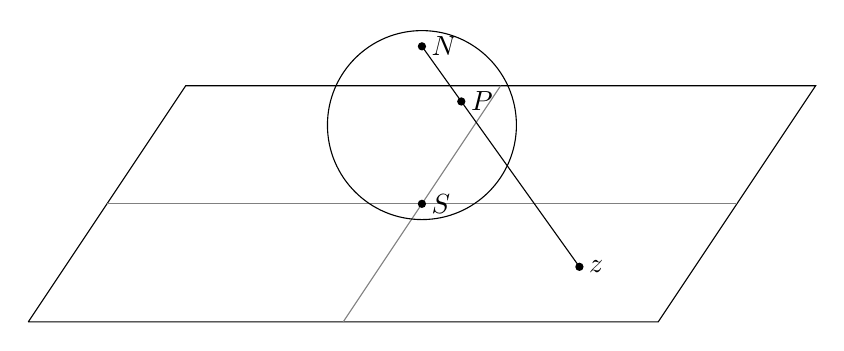
\begin{tikzpicture}
    \draw (0, 0) -- (8, 0) -- (10, 3) -- (2, 3) -- (0, 0);
    \draw [gray] (1, 1.5) -- (9, 1.5);
    \draw [gray] (4, 0) -- (6, 3);
    \draw (5, 2.5) circle [radius=1.2];

    \node [circ] at (5, 1.5) {};
    \node at (5, 1.5) [right] {$S$};

    \node [circ] at (5, 3.5) {};
    \node at (5, 3.5) [right] {$N$};

    \node [circ] at (5.5, 2.8) {};
    \node at (5.5, 2.8) [right] {$P$};

    \draw (5, 3.5) -- (7, 0.7) node [circ] {} node [right] {$z$};
  \end{tikzpicture}
\end{center}
 % improve
For any point $z \in \C$, drawing a line through the ``North Pole'' $N$ of the sphere to $z$, and noting where this intersects the sphere. This specifies an equivalent point $P$ on the sphere. Then $\infty$ is equivalent to the North Pole of the sphere itself. So the extended complex plane is mapped bijectively to the sphere.

To investigate properties of $\infty$, we use the substitution $\zeta = \frac{1}{z}$. A function $f(z)$ is said to have a particular property \emph{at $\infty$} if $f(\frac{1}{\zeta})$ has that same property at $\zeta = 0$. This vague notion will be made precise when we have specific examples to play with.

\subsection{Complex differentiation}
Recall the definition of differentiation for a real function $f(x)$:
\[
  f'(x) = \lim_{\delta x \to 0} \frac{f(x + \delta x) - f(x)}{\delta x}.
\]
It is implicit that the limit must be the same whichever direction we approach from. For example, consider $|x|$ at $x = 0$. If we approach from the right, ie. $\delta x \to 0^+$, then the limit is $+1$, whereas from the left, ie. $\delta x \to 0^-$, the limit is $-1$. Because these limits are different, we say that $|x|$ is not differentiable at the origin.

This is obvious and we already know that, but for complex differentiation, this issue is much more important, since there are many more directions. We now extend the definition of differentiation to complex number:
\begin{defi}[Complex differentiable function]
  A complex differentiable function $f: \C \to \C$ is \emph{differentiable} at $z$ if
  \[
    f'(z) = \lim_{\delta z \to 0} \frac{f(z + \delta z) - f(z)}{\delta z}
  \]
  exists (and is therefore independent of the direction of approach --- but now there are infinitely many possible directions).
\end{defi}

\begin{defi}[Analytic function]
  We say $f$ is \emph{analytic} at a point $z$ if there exists a neighbourhood of $z$ throughout which $f'$ exists. The terms \emph{regular} and \emph{holomorphic} are also used.
\end{defi}
In complex analysis, this sentence might be a few paragraphs long instead. Usually ``holomorphic'' is defined to mean the function has a Taylor series, but then we go on to prove that having a Taylor series is the same as being differentiable in a neighbourhood, ie. being holomorphic and analytic are the same.

\begin{defi}[Entire function]
  A complex function is \emph{entire} if it is analytic throughout $\C$.
\end{defi}

The property of analyticity is in fact a surprisingly strong one! For example, two consequences are:
\begin{enumerate}
  \item If a function is analytic, then it is differentiable infinitely many times. This is very \emph{very} false for real functions. There are real functions differentiable $N$ times, but no more (eg. by taking a non-differentiable function and integrating it $N$ times).
  \item A bounded entire function must be a constant.
\end{enumerate}
There are many more interesting properties, but these are sufficient to show us that complex differentiation is very different from real differentiation.
\subsubsection*{The Cauchy-Riemann equations}
We start by separating $f$ and $z$ into real and imaginary parts, ie.
\[
  f(z) = u(x, y) + iv(x, y),
\]
where $z = x + iy$ are $u, v$ are real functions.

We suppose that $f$ is differentiable at $z$. We may take $\delta z$ in any direction we like. First, we take it to be real, with $\delta z = \delta x$. Then
\begin{align*}
  f'(z) &= \lim_{\delta x \to 0} \frac{f(z + \delta x) - f(z)}{\delta x}\\
  &= \lim_{\delta x \to 0} \frac{u(x + \delta x, y) + iv(x + \delta x, y) - (u(x, y) + iv(x, y))}{\delta x}\\
  &= \frac{\partial u}{\partial x} + i \frac{\partial v}{\partial x}.
\end{align*}
What this says is something entirely obvious --- since we are allowed to take the limit in any direction, we can take it in the $x$ direction, and we get the corresponding partial derivative. This is a completely uninteresting point. Instead, let's do the really fascinating thing of taking the limit in the $y$ direction!

Let $\delta z = i \delta y$. Then we can compute
\begin{align*}
  f'(z) &= \lim_{\delta y \to 0} \frac{f(z + i\delta y) - f(z)}{i \delta y}\\
  &= \lim_{\delta y \to 0} \frac{u(x, y + \delta y) + iv(x, y + \delta y) - (u(x, y) + iv(x, y))}{i \delta y}\\
  &= \frac{\partial v}{\partial y} - i \frac{\partial u}{\partial y}.
\end{align*}
By the definition of differentiability, the two results for $f'(z)$ must agree! So we must have
\[
  \frac{\partial u}{\partial x} + i \frac{\partial v}{\partial x} = \frac{\partial v}{\partial y} - i \frac{\partial u}{\partial y}.
\]
Taking the real and imaginary components, we get
\begin{prop}[Cauchy-Riemann equations]
  If $f = u + iv$ is differentiable, then
  \[
    \frac{\partial u}{\partial x} = \frac{\partial v}{\partial y},\quad \frac{\partial u}{\partial y} = -\frac{\partial v}{\partial x}.
  \]
\end{prop}
Is the converse true? If these equations hold, does it follow that $f$ is differentiable? This is not always true. This holds only if $u$ and $v$ themselves are differentiable, which is a stronger condition that the partial derivatives exist, as you may have learnt from IB Analysis II. In particular, this holds if the partial derivatives $u_x, u_y, v_x, v_y$ are continuous (which implies differentiability).

\subsubsection*{Examples of analytic functions}
\begin{eg}\leavevmode
  \begin{enumerate}
    \item $f(z) = z$ is entire, ie. differentiable everywhere. Here $u = x, v = y$. Then the Cauchy-Riemann equations are satisfied everywhere, since
      \[
        \frac{\partial u}{\partial x} = \frac{\partial v}{\partial y} = 1,\quad \frac{\partial u}{\partial y} = -\frac{\partial v}{\partial x} = 0,
      \]
      and these are clearly continuous. Alternatively, we can prove this directly from the definition.
    \item $f(z) = e^z = e^x (\cos y + i \sin y)$ is entire since
      \[
        \frac{\partial u}{\partial x} = e^x \cos y = \frac{\partial v}{\partial y},\quad \frac{\partial u}{\partial y} = - e^x \sin y = -\frac{\partial v}{\partial x}.
      \]
      The derivative is
      \[
        f'(z) = \frac{\partial u}{\partial x} + i \frac{\partial v}{\partial x} = e^x \cos y + i e^x \sin y = e^z,
      \]
      as expected.
    \item $f(z) = z^n$ for $n \in \N$ is entire. This is less straightforward to check. Writing $z = r(\cos \theta + i \sin \theta)$, we obtain
      \[
        u = r^n \cos n\theta,\quad v = r^n \sin n\theta.
      \]
      We can check the Cauchy-Riemann equation using the chain rule, writing $r = \sqrt{x^2 = y^2}$ and $\tan \theta = \frac{y}{x}$. This takes quite a while, and it's not worth your time. But if you really do so, you will find the derivative to be $nz^{n - 1}$.
    \item Any rational function, ie. $f(z) = \frac{P(z)}{Q(z)}$ where $P, Q$ are polynomials, is analytic \emph{except} at points where $Q(z) = 0$ (where it is not even defined). For instance,
      \[
        f(z) = \frac{z}{z^2 + 1}
      \]
      is analytic except at $\pm i$.
    \item Many standard functions can be extended naturally to complex functions and obey the usual rules for their derivatives. For example,
      \begin{itemize}
        \item $\sin z = \frac{e^{iz} - e^{-iz}}{2i}$ is differentiable with derivative $\cos z = \frac{e^{iz} + e^{-iz}}{2}$. We can also write
          \begin{align*}
            \sin z &= \sin (x + iy) \\
            &= \sin x \cos iy + \cos x \sin iy \\
            &= \sin x \cosh y + i \cos x \sinh y.
          \end{align*}
        \item Similarly $\cos z, \sinh z, \cosh z$ etc. differentiate to what we expect them to differentiate to.
        \item $\log z = \log|z| + i \arg z$ has derivative $\frac{1}{z}$.
        \item The product rule, quotient rule and chain rule hold in exactly the same way, which allows us to prove (iii) and (iv) easily.
      \end{itemize}
  \end{enumerate}
\end{eg}

\subsubsection*{Examples of non-analytic functions}
\begin{eg}\leavevmode
  \begin{enumerate}
    \item Let $f(z) = \Re z$. This has $u = x, v = 0$. But
      \[
        \frac{\partial u}{\partial x} = 1\not= 0 = \frac{\partial v}{\partial y}.
      \]
      So $\Re z$ is nowhere analytic.
    \item Consider $f(z) = |z|$. This has $u = \sqrt{x^2 + y^2} = 0, v = 0$. This is thus nowhere analytic.
    \item The complex conjugate $f(z) = \bar z = z^* = x - iy$ has $u = x, v = -y$. So the Cauchy-Riemann equations don't hold. Hence this is nowhere analytic.

      We could have deduced (ii) from this --- if $|z|$ were analytic, then so would $|z|^2$, and hence $\bar{z} = \frac{|z|^2}{z}$ also has to be analytic.
    \item We have to be a bit more careful with $f(z) = |z|^2 = x^2 + y^2$. The Cauchy-Riemann equations are satisfied only at the origin. So $f$ is only differentiable at $z = 0$. However, it is not analytic since there is no neighbourhood of $0$ throughout which $f$ is differentiable.
  \end{enumerate}
\end{eg}

\subsection{Harmonic functions}
This is the last easy section of the course.

\begin{defi}[Harmonic conjugates]
  Functions $u, v$ satisfying the Cauchy-Riemann equations are called \emph{harmonic conjugates}.
\end{defi}

If we know one, then we can find the other up to a constant. For example, if $u(x, y) = x^2 - y^2$, then $v$ must satisfy
\[
  \frac{\partial v}{\partial y} = \frac{\partial u}{\partial x} = 2x.
\]
So we must have $v = 2xy + g(x)$ for some function $g(x)$. The other Cauchy-Riemann equation gives
\[
  -2y = \frac{\partial u}{\partial y} = -\frac{\partial v}{\partial x} = -2y - g'(x).
\]
This tells us $g'(x) = 0$. So $g$ must be a genuine constant, say $\alpha$. The corresponding analytic function whose real part is $u$ is therefore
\[
  f(z) = x^2 - y^2 + 2ixy + i\alpha = (x + iy)^2 + i \alpha = z^2 + i\alpha.
\]
Note that in an exam, if we were asked to find the analytic function $f$ with real part $u$ (where $u$ is given), then we \emph{must} express it in terms of $z$, and not $x$ and $y$, or else it is not clear this is indeed analytic.

On the other hand, if $f(z) = u + iv$ is analytic, then we can compute
\begin{align*}
  \frac{\partial^2 u}{\partial x^2} &= \frac{\partial }{\partial x}\left(\frac{\partial u}{\partial x}\right)\\
  &= \frac{\partial }{\partial x} \left(\frac{\partial v}{\partial y}\right)\\
  &= \frac{\partial }{\partial y}\left(\frac{\partial v}{\partial x}\right)\\
  &= \frac{\partial }{\partial y}\left(- \frac{\partial u}{\partial y}\right)\\
  &= -\frac{\partial^2 u}{\partial y^2}.
\end{align*}
So $u$ satisfies Laplace's equation in two dimensions, ie.
\[
  \nabla^2 u = \frac{\partial^2 u}{\partial x^2} + \frac{\partial^2 u}{\partial y^2} = 0.
\]
Similarly, so does $v$.
\begin{defi}[Harmonic function]
  A function satisfying Laplace's equation equation in an open set is said to be \emph{harmonic}.
\end{defi}

Thus we have shown the following:
\begin{prop}
  The real and imaginary parts of any analytic function are harmonic.
\end{prop}

\subsection{Multi-valued functions}
For $z = r^{i\theta}$, we define $\log z = \log r + i \theta$. There are infinitely many values of $\log z$, for every choice of $\theta$. For example,
\[
  \log i = \frac{\pi i}{2} \text{ or }\frac{5\pi i}{2}\text{ or } -\frac{3\pi i}{2}\text{ or }\cdots.
\]
This is fine, right? Functions can be multi-valued. Nothing's wrong.
\end{document}
